\section{Analysis Classes}

In our application we can distinguish three analysis classes. The name of each
class is self explanatory. As we can see from the diagram in
Figure~\ref{fig:classes} these classes are associated in the following way:

\begin{enumerate}
	\item Users can be divided in Owners and Customers.
	\item Each Owner can have one and only one Restaurant.
	\item Each Customer can have none or many Reservations.
	\item Each Restaurant must have one and only one Owner associated.
	\item Each Restaurant can have none or many Reservations.
	\item Each Reservation can be associated to one and only one Customer.
	\item Each Reservation can be associated to one and only one Restaurant.
\end{enumerate}

\begin{figure}[ht]
	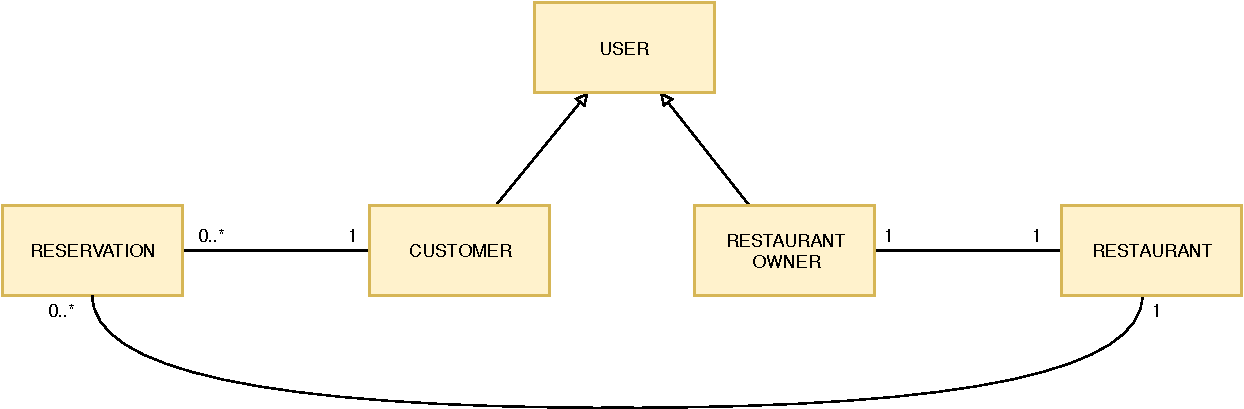
\includegraphics[width=\textwidth]{classes}
	\caption{Analysis classes diagram.}
	\label{fig:classes}
\end{figure}
